\chapter{激光：受激辐射与高斯光束}\label{ch:b2:laser}

讲台屏幕上的红点、收银台的条形码读取器、
读取光盘的光束、焊接车身的光束、穿越海底承载互联网的光束、
矫正角膜的光束，以及精确到毫米测量至月球距离的光束：
这些都是\emph{激光}，即一种
有别于任何火焰或灯具的光源。它的光在十亿分之一的范围内呈单一颜色，
在整个房间内保持毫米量级的光束，并可
聚焦成宽仅几个波长的光斑，此时其辐照度
可超过太阳表面辐照度的百万倍。这一切并非源于
某种新型原子，而来自爱因斯坦于 1917 年揭示的一个过程
——\emph{\omterm{def:b2:laser:processes}{受激辐射}}，即发射一个与
已有光子完全相同的光子——以及让物质处于使这一过程
胜过\omterm{def:b2:laser:processes}{吸收}，然后把放大器置于两面镜子之间，
使其自我\omterm{def:b2:feedback-oscillators:loop}{反馈}。本章分三步建立激光理论：
光与原子群如何交换能量（\omterm{def:b2:laser:processes}{爱因斯坦
系数}），何时交换会产生放大（\omterm{prop:b2:laser:gain}{粒子数反转}与增益），
增益），以及放大器何时成为振荡器（谐振腔、
其阈值与模式）。全章以射出光束的形状收尾——
即\omterm{prop:b2:laser:gaussian}{高斯光束}，其\omterm{prop:b2:laser:gaussian}{束腰}与发散角
决定了激光在远处和焦点处能做什么。

\begin{omfigure}
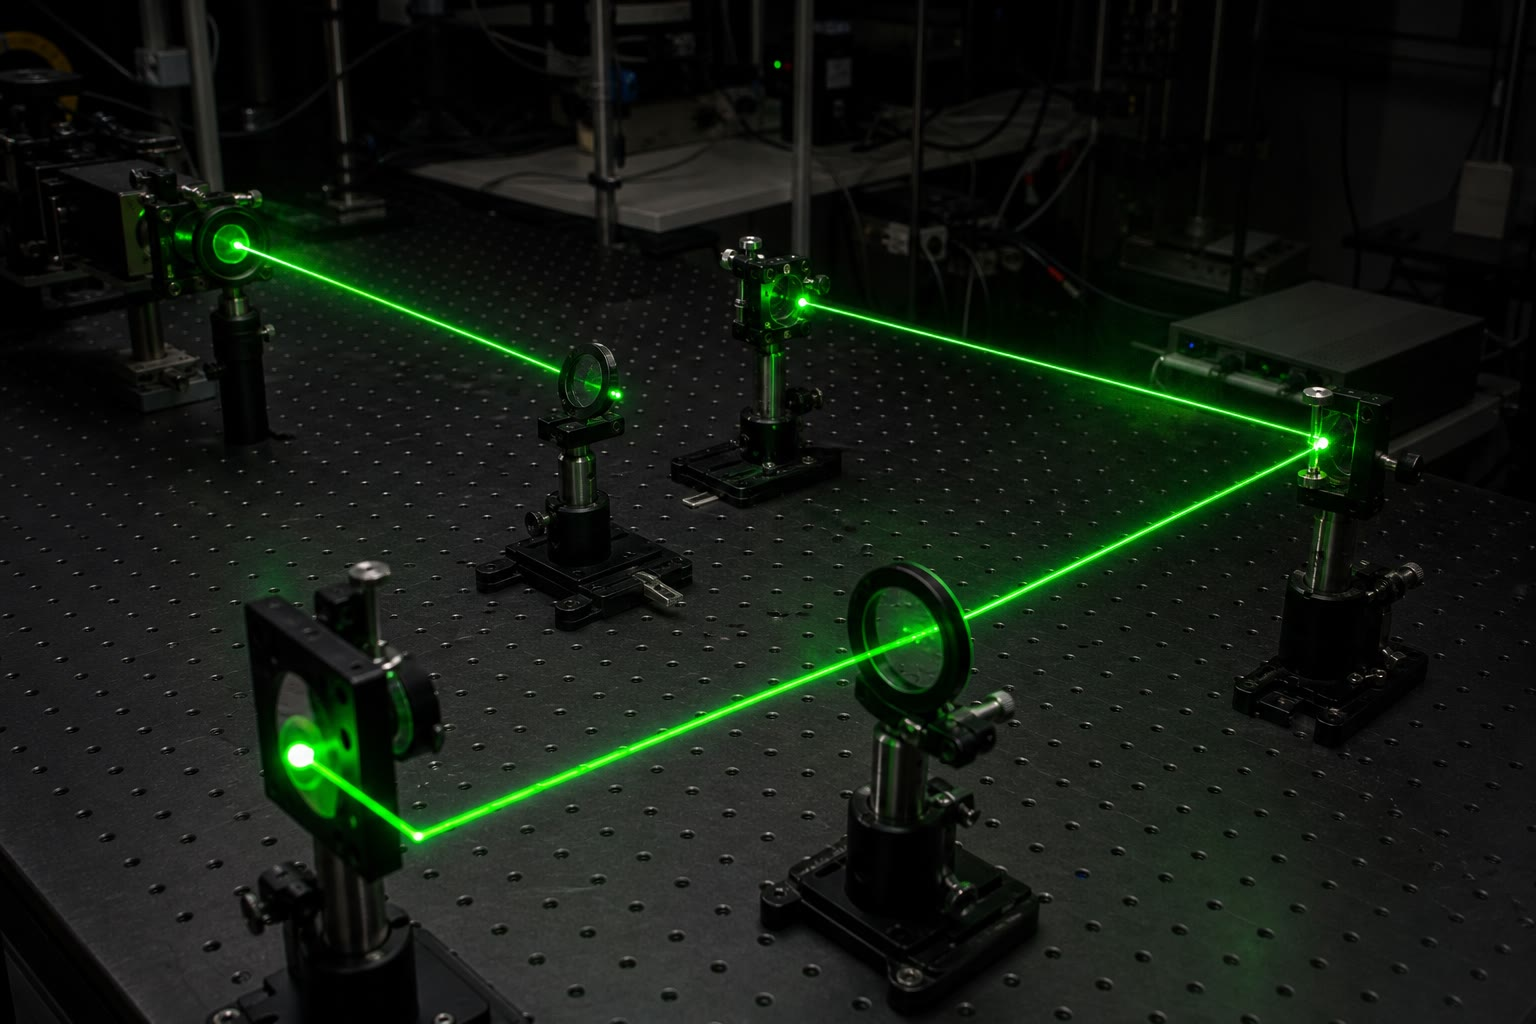
\includegraphics[width=0.58\linewidth]{images/book4/ai/b4-23-laser-optical-table.jpg}

{\small 光学平台：\omterm{def:b2:laser:cavity}{激光器}、镜子、透镜，以及始终
保持为贯穿整个房间的细线光束——这是灯具无法具备的
方向性。}
\end{omfigure}

\section{光与物质：三种过程}

\begin{definition}[吸收、自发辐射与受激辐射]\label{def:b2:laser:processes}
考虑具有两个能级 $E_1 < E_2$ 的原子，其粒子数（数密度）
分别为 $N_1$、$N_2$，以及频率为 $\nu$ 的光，满足
$h\nu = E_2 - E_1$，光谱能量密度为 $u(\nu)$（单位体积、单位频率内的
能量）。三种过程交换能量：
\begin{itemize}
\item \emph{吸收}\index{吸收（光）}：
      $E_1$ 的原子吸收一个光子，跃迁至 $E_2$，
      单位体积、单位时间内的速率为 $B_{12}\,u(\nu)\,N_1$；
\item \emph{自发辐射}\index{自发辐射}：处于
      $E_2$ 的原子自发跃迁回 $E_1$，发射一个方向任意、相位随机的光子，
      速率为 $A_{21}N_2$——
      $1/A_{21} = \tau$ 即该能级的寿命；
\item \emph{受激辐射}\index{受激辐射}：一个频率为
      $\nu$ 的光子经过处于 $E_2$ 的原子时，诱使其跃迁回落，
      发射出一个与原光子\emph{完全相同}的光子（频率、方向、
      相位与偏振均相同），速率为
      $B_{21}\,u(\nu)\,N_2$。
\end{itemize}
$A_{21}$、$B_{12}$、$B_{21}$ 称为该跃迁的\emph{爱因斯坦
系数}\index{爱因斯坦系数}。
\end{definition}

\begin{proposition}[爱因斯坦关系]\label{prop:b2:laser:einstein}
对于非简并能级，
\[
B_{12} = B_{21} \equiv B, \qquad
\frac{A_{21}}{B_{21}} = \frac{8\pi h\nu^3}{c^3}.
\]
\omterm{def:b2:laser:processes}{受激辐射}与\omterm{def:b2:laser:processes}{吸收}具有相同的系数；
\omterm{def:b2:laser:processes}{自发辐射}速率相对\omterm{def:b2:laser:processes}{受激辐射}速率按 $\nu^3$ 的规律增长。
\end{proposition}

\begin{proof}
设原子与温度为 $T$ 的辐射处于平衡。下面两个事实
取自后文：平衡时两能级的粒子数之比
为 $N_2/N_1 = \eu^{-h\nu/k_BT}$（
玻尔兹曼因子，见\cref{ch:b2:boltzmann-factor}），平衡辐射
的光谱密度具有普朗克形式
$u(\nu) = (8\pi h\nu^3/c^3)/(\eu^{h\nu/k_BT} - 1)$
（见\cref{ch:b2:thermal-radiation}）。平衡时各能级的粒子数保持稳定，
即 $B_{12}uN_1 = A_{21}N_2 + B_{21}uN_2$，由此
\[
u = \frac{A_{21}}{B_{12}\,N_1/N_2 - B_{21}}
  = \frac{A_{21}}{B_{12}\eu^{h\nu/k_BT} - B_{21}}.
\]
这一结果须对每个 $T$ 都与普朗克表达式一致：$T \to \infty$
的极限（此时 $u \to \infty$）迫使 $B_{12} = B_{21}$，而
比较即得 $A_{21}/B_{21} = 8\pi h\nu^3/c^3$。
系数是原子本身的性质，因此这些关系
在非平衡状态下同样成立。
\end{proof}

\begin{remark}[为什么灯不能放大]\label{rem:b2:laser:lamps}
在 \qty{300}{K} 的气体中，对于可见光跃迁（$h\nu \approx
\qty{2}{eV}$，$k_BT \approx \qty{0.025}{eV}$），$N_2/N_1 = \eu^{-80} \approx
10^{-35}$：几乎没有原子被激发，光只会被\omterm{def:b2:laser:processes}{吸收}。
放电或火焰能使 $E_2$ 有粒子布居，但仍是 $N_2 < N_1$，
每个发射的光子都被更多的\omterm{def:b2:laser:processes}{吸收}所压制；此外，
平衡时\omterm{def:b2:laser:processes}{自发辐射}与\omterm{def:b2:laser:processes}{受激辐射}之比
$A_{21}/(B_{21}u) = \eu^{h\nu/k_BT} - 1$，在
可见光波段大得惊人——灯光是自发的：相位随机、
各方向皆有，占满整条谱线的宽度。仅在无线电与微波
频段（$h\nu \ll k_BT$）时，\omterm{def:b2:laser:processes}{受激辐射}才能自然地参与竞争；
第一台此类器件确为微波激射器，其工作频率为
\qty{24}{GHz}（1954 年），早于光学\omterm{def:b2:laser:cavity}{激光器}（1960 年）。
\end{remark}

\begin{omfigure}
\begin{tikzpicture}[scale=0.9, >=stealth]
  \foreach \x/\t in {0/吸收, 3.6/自发辐射, 7.2/受激辐射}{
    \draw[thick] (\x,0) -- ++(2,0) node[right, font=\scriptsize] {$E_1$};
    \draw[thick] (\x,1.6) -- ++(2,0) node[right, font=\scriptsize] {$E_2$};
    \node[font=\scriptsize, align=center] at (\x+1,-0.5) {\t};
  }
  % absorption
  \fill (1,0) circle (2pt);
  \draw[->, omDef, thick] (1,0.15) -- (1,1.45);
  \draw[->, omExo, thick, decorate, decoration={snake, amplitude=0.6mm, segment length=2mm}] (-0.6,0.8) -- (0.7,0.8);
  \node[font=\scriptsize, omExo] at (-0.5,1.15) {$h\nu$};
  % spontaneous
  \fill (4.6,1.6) circle (2pt);
  \draw[->, omDef, thick] (4.6,1.45) -- (4.6,0.15);
  \draw[->, omExo, thick, decorate, decoration={snake, amplitude=0.6mm, segment length=2mm}] (4.8,0.8) -- (6.2,1.3);
  % stimulated
  \fill (8.2,1.6) circle (2pt);
  \draw[->, omDef, thick] (8.2,1.45) -- (8.2,0.15);
  \draw[->, omExo, thick, decorate, decoration={snake, amplitude=0.6mm, segment length=2mm}] (6.6,0.8) -- (7.9,0.8);
  \draw[->, omExo, thick, decorate, decoration={snake, amplitude=0.6mm, segment length=2mm}] (8.5,0.95) -- (9.9,0.95);
  \draw[->, omExo, thick, decorate, decoration={snake, amplitude=0.6mm, segment length=2mm}] (8.5,0.65) -- (9.9,0.65);
  \node[font=\scriptsize, omExo] at (10.6,0.8) {$2h\nu$};
\end{tikzpicture}

{\small 两能级之间的三种过程：\omterm{def:b2:laser:processes}{吸收}使一个光子消失；
\omterm{def:b2:laser:processes}{自发辐射}产生一个相位和方向随机的光子；
\omterm{def:b2:laser:processes}{受激辐射}产生一个与入射光子完全相同的光子，
即一个副本。}
\end{omfigure}

\section{放大：粒子数反转与增益}

\begin{proposition}[介质的增益]\label{prop:b2:laser:gain}
光强为 $I$、频率为 $\nu$ 的光束穿过介质时，
通过\omterm{def:b2:laser:processes}{受激辐射}获得能量，通过\omterm{def:b2:laser:processes}{吸收}损失能量
（\omterm{def:b2:laser:processes}{自发辐射}向各个方向发出，几乎不对
光束有贡献）。在长度 $\dd z$ 内，
\[
\dd I = \sigma\,(N_2 - N_1)\,I\,\dd z, \qquad
I(z) = I(0)\,\eu^{g z}, \qquad g = \sigma(N_2 - N_1),
\]
其中 $\sigma$（面积，即跃迁的\emph{截面}\index{截面 }
，$\sigma \propto B\,h\nu/c$）刻画跃迁的
强度。介质\emph{放大}光束（$g > 0$）
只有当
\[
N_2 > N_1 :
\]
时，即\emph{粒子数反转}\index{粒子数反转}。无此条件时
（$N_2 < N_1$，即一切处于平衡态的介质的情形），光束
被\omterm{def:b2:laser:processes}{吸收}。
\end{proposition}

\begin{proof}
单位体积、单位时间内，$B u (N_2 - N_1)$ 次跃迁
为光束增加（或减少）一个光子 $h\nu$；取 $u = I/c$（单位频率，
对谱线宽度积分），单位体积获得的功率为
$B h\nu (N_2 - N_1) I/c$，即 $\dd I/\dd z$；定义 $\sigma =
Bh\nu/c$（乘以线形因子）。
\end{proof}

\begin{remark}[两能级体系为何不能反转]\label{rem:b2:laser:twolevel}
用频率为 $\nu$ 的光对两能级体系施以任意强的抽运：
抽运光在 $N_1 > N_2$ 时被\omterm{def:b2:laser:processes}{吸收}，在 $N_2 > N_1$ 时引起\omterm{def:b2:laser:processes}{受激辐射}，
粒子数至多趋于相等，$N_2 = N_1$，此时
介质透明但无增益。反转至少需要
三个能级：抽运将粒子从基态激发到寿命短的能级，该能级
迅速衰变到上激光能级，后者为\emph{长寿命}
（亚稳态），因而能积累粒子。在
\emph{三能级}\index{三能级}方案（红宝石，第一台
\omterm{def:b2:laser:cavity}{激光器}）中，下激光能级即为基态，因此须先将超过一半的原子
激发，才能实现反转：抽运十分剧烈。在
\emph{四能级}\index{四能级}方案（He--Ne、Nd:YAG 等，多数
\omterm{def:b2:laser:cavity}{激光器}）中，下激光能级是一个会迅速排空到基态的激发态；
该能级几乎始终无粒子，因此上能级中的少量粒子
便已构成反转——阈值
很低。
\end{remark}

\begin{omfigure}
\begin{tikzpicture}[scale=0.85, >=stealth]
  % three-level
  \draw[thick] (0,0) -- (2,0) node[right, font=\scriptsize] {$0$：基态};
  \draw[thick] (0,2.4) -- (2,2.4) node[right, font=\scriptsize] {$2$（寿命短）};
  \draw[thick] (0,1.8) -- (2,1.8) node[right, font=\scriptsize] {$1$（亚稳态）};
  \draw[->, omExo, thick] (0.5,0.05) -- (0.5,2.35) node[midway, left, font=\scriptsize] {抽运};
  \draw[->, dashed] (1.0,2.35) -- (1.0,1.85);
  \draw[->, omDef, very thick] (1.5,1.75) -- (1.5,0.05) node[midway, right, font=\scriptsize] {激光};
  \node[font=\scriptsize] at (1.8,-0.6) {三能级（红宝石）};
  % four-level
  \begin{scope}[xshift=7cm]
  \draw[thick] (0,0) -- (2,0) node[right, font=\scriptsize] {$0$：基态};
  \draw[thick] (0,2.4) -- (2,2.4) node[right, font=\scriptsize] {$3$（寿命短）};
  \draw[thick] (0,1.9) -- (2,1.9) node[right, font=\scriptsize] {$2$（亚稳态）};
  \draw[thick] (0,0.6) -- (2,0.6) node[right, font=\scriptsize] {$1$（迅速排空）};
  \draw[->, omExo, thick] (0.5,0.05) -- (0.5,2.35) node[midway, left, font=\scriptsize] {抽运};
  \draw[->, dashed] (1.0,2.35) -- (1.0,1.95);
  \draw[->, omDef, very thick] (1.5,1.85) -- (1.5,0.65) node[midway, right, font=\scriptsize] {激光};
  \draw[->, dashed] (1.0,0.55) -- (1.0,0.05);
  \node[font=\scriptsize] at (1.8,-0.6) {四能级（He--Ne、Nd:YAG）};
  \end{scope}
\end{tikzpicture}

{\small 抽运方案。左：三能级——激光跃迁
终止于基态，基态须被抽空一半以上。右：
四能级——下激光能级立即排空至基态，
因此上能级的少量粒子便已构成反转。}
\end{omfigure}

\begin{proposition}[增益的饱和]\label{prop:b2:laser:saturation}
反转由抽运维持，抽运以单位体积速率 $R$ 向上能级
供给粒子，并抗衡衰减 $1/\tau$ 与
\omterm{def:b2:laser:processes}{受激辐射} $\sigma I (N_2 - N_1)/h\nu$。在四能级
介质（$N_1 \approx 0$）中，稳态为
\[
N_2 = \frac{R\tau}{1 + I/I_{\text{s}}}, \qquad
g = \frac{g_0}{1 + I/I_{\text{s}}}, \qquad
I_{\text{s}} = \frac{h\nu}{\sigma\tau} :
\]
\emph{小信号增益} $g_0 = \sigma R\tau$ 会被光束本身
削弱：一旦 $I$ 接近\emph{饱和
光强}\index{饱和光强} $I_{\text{s}}$ 时，放大器
呈非线性，这种非线性恰恰决定
\omterm{def:b2:laser:cavity}{激光器}功率的大小。
\end{proposition}

\begin{proof}
$\dd N_2/\dd t = R - N_2/\tau - \sigma I N_2/h\nu = 0$.
\end{proof}

\section{振荡器：谐振腔、阈值与模式}

\begin{definition}[激光谐振腔]\label{def:b2:laser:cavity}
\emph{激光器}\index{激光器}是一段长度为 $\ell$ 的放大介质，
置于两面反射镜（反射率为 $R_1$、$R_2$）之间，
相距 $L$，构成法布里–珀罗腔（\cref{ch:b2:gratings}）。
\emph{输出耦合镜}为部分透射镜（$T_2 = 1 - R_2$ 约为
百分之几），使光束射出。在谐振腔中绕行的光
经介质两次放大，并因反射镜及
其他损耗（散射、\omterm{def:b2:laser:processes}{吸收}、\omterm{def:b2:diffraction:huygens}{衍射}）而衰减。
\end{definition}

\begin{theorem}[振荡条件]\label{thm:b2:laser:threshold}
复振幅为 $\underline s$ 的波
经一次往返后能重现自身的条件是
\[
\underline s\,\cdot\, \eu^{g\ell}\sqrt{R_1}\,\eu^{g\ell}\sqrt{R_2}\,
\eu^{-\alpha\cdot 2L}\,\eu^{2\iu kL} = \underline s
\]
（$\alpha$：单位长度的其他损耗）。由此得两个条件。
\begin{itemize}
\item \emph{振幅条件}：$R_1R_2\,\eu^{2(g\ell - \alpha L)} \ge 1$，即
      增益必须达到\emph{阈值}\index{阈值（激光）}
      \[
      g_{\text{阈}} = \frac{1}{\ell}\Big(\alpha L - \tfrac12\ln(R_1R_2)\Big)
      \approx \frac{1}{2\ell}\,(T_2 + \text{每次往返的损耗}) ;
      \]
\item \emph{相位条件}：$2kL = 2\pi p$，即 $\nu_p = p\,c/2L$——\omterm{def:b2:laser:cavity}{激光器}只在
      谐振腔的\emph{纵模}\index{纵模}
上振荡，相邻纵模间隔为 $c/2L$，其中只有
      位于增益曲线之下且满足 $g(\nu) \ge g_{\text{阈}}$ 的那些模式才振荡。
\end{itemize}
\end{theorem}

\begin{proof}
往返因子的振幅与相位都须为平凡的；近似
中用到了 $-\ln R \approx 1 - R = T$，适用于 $T \ll 1$ 的情形。
\end{proof}

\begin{proposition}[阈值以上的稳态]\label{prop:b2:laser:steady}
从单个原子的\omterm{def:b2:laser:processes}{自发辐射}出发，对任一满足
$g_0 > g_{\text{阈}}$ 的模式会按每次往返指数增长；
随其强度增大，增益饱和
（见\cref{prop:b2:laser:saturation}）直至恰与损耗相等：
\[
g(I) = g_{\text{阈}} \quad\Longrightarrow\quad
I_{\text{谐振腔}} = I_{\text{s}}\Big(\frac{g_0}{g_{\text{阈}}} - 1\Big),
\qquad P_{\text{出}} = T_2\,I_{\text{谐振腔}}\,A .
\]
增益\emph{钳位}于阈值；每个额外泵浦到阈值以上的
原子都变为一个输出光子，因此输出功率
随超过阈值泵浦量线性增长。
\end{proposition}

\begin{remark}[激光器是一种反馈振荡器]\label{rem:b2:laser:feedback}
可将\omterm{def:b2:laser:cavity}{激光器}与\omterm{prop:b2:feedback-oscillators:wien}{维恩电桥振荡器}相比较，
参见\cref{ch:b2:feedback-oscillators}：一个放大器（即反转介质），
一个选频\omterm{def:b2:feedback-oscillators:loop}{反馈}（谐振腔，只让其模式通过），
一个起振条件（\omterm{def:b2:feedback-oscillators:loop}{环路增益} $> 1$，即 $g_0 > g_{\text{阈}}$），
从噪声起振（此处为\omterm{def:b2:laser:processes}{自发辐射}），以及由放大器的非线性
（增益饱和）所决定的振幅。\omterm{def:b2:laser:cavity}{激光器}是该族的
光学成员。
\end{remark}

\begin{omfigure}
\begin{tikzpicture}
  \begin{axis}[omaxis, width=8.2cm, height=4.6cm, xmin=-2.4, xmax=2.4, ymin=0, ymax=1.25,
    xlabel={$(\nu - \nu_0)/\Delta\nu$}, ylabel={$g(\nu)$}, ytick=\empty,
    xtick={-2,-1,0,1,2}, clip=false]
    \addplot[omDef, thick, domain=-2.4:2.4, samples=120] {exp(-2.77*x*x)};
    \addplot[omExo, thick, dashed, domain=-2.4:2.4] {0.45};
    \node[font=\scriptsize, omExo, anchor=west] at (axis cs:1.6,0.55) {$g_{\text{阈}}$};
    \draw[gray!70] (axis cs:-1.75,0) -- (axis cs:-1.75,0.12);
    \draw[gray!70] (axis cs:-1.4,0) -- (axis cs:-1.4,0.12);
    \draw[gray!70] (axis cs:-1.05,0) -- (axis cs:-1.05,0.12);
    \draw[gray!70] (axis cs:-0.7,0) -- (axis cs:-0.7,0.12);
    \draw[gray!70] (axis cs:0.7,0) -- (axis cs:0.7,0.12);
    \draw[gray!70] (axis cs:1.05,0) -- (axis cs:1.05,0.12);
    \draw[gray!70] (axis cs:1.4,0) -- (axis cs:1.4,0.12);
    \draw[gray!70] (axis cs:1.75,0) -- (axis cs:1.75,0.12);
    \draw[omThm, very thick] (axis cs:-0.35,0) -- (axis cs:-0.35,0.712);
    \draw[omThm, very thick] (axis cs:0,0) -- (axis cs:0,1.000);
    \draw[omThm, very thick] (axis cs:0.35,0) -- (axis cs:0.35,0.712);
    \node[font=\scriptsize, anchor=south] at (axis cs:-1.4,0.14) {$c/2L$};
    \draw[<->, thin] (axis cs:-1.75,0.12) -- (axis cs:-1.05,0.12);
  \end{axis}
\end{tikzpicture}

{\small 介质的增益曲线（宽度 $\Delta\nu$）、由损耗确定的阈值，
以及间距为 $c/2L$ 的谐振腔模式梳：只有
位于曲线之下且高于阈值（粗线所示）的模式才振荡。}
\end{omfigure}

\begin{example}[氦氖激光器]\label{ex:b2:laser:hene}
一根玻璃管长 \qty{30}{cm}、内径 \qty{1}{mm}，内充氦和
氖，气压约为一个大气压的千分之一，管中通有
几毫安的放电电流。电子将氦激发到亚稳态，能量为
\qty{20.6}{eV}，通过碰撞将其能量传给一个
几乎同高度的氖能级；氖原子由此衰变到较低能级
（迅速跃迁到基态——四能级），通过辐射发出
\qty{632.8}{nm} 的光。小信号增益很小，每程仅百分之几，
因此反射镜必须非常优良（$R_1 = 0.999$，$R_2 = 0.99$），
管子也须洁净；增益线经多普勒展宽至
$\Delta\nu \approx \qty{1.5}{GHz}$，纵模间隔为 $c/2L = \qty{500}{MHz}$，
因此同时有两个或三个纵模振荡。输出 \qty{1}{mW}，对应
数瓦放电功率，效率为 $10^{-4}$；但波长
可确定至 $10^{-6}$，光束在整个
实验室中始终保持 \qty{1}{mm} 宽。
\end{example}

\section{高斯光束}

\begin{proposition}[高斯光束]\label{prop:b2:laser:gaussian}
由带曲面镜的稳定谐振腔发出的光束（处于
基横模）为\emph{高斯光束}\index{高斯光束}
：距其最窄截面为 $z$ 处（即
\emph{束腰}\index{束腰（光束）}，半径为 $w_0$）的光强
分布为
\[
I(r,z) = \frac{2P}{\pi w(z)^2}\,\exp\Big(-\frac{2r^2}{w(z)^2}\Big),
\qquad
w(z) = w_0\sqrt{1 + \Big(\frac{z}{z_{\text{R}}}\Big)^2},
\qquad
z_{\text{R}} = \frac{\pi w_0^2}{\lambda},
\]
其中 $P$ 为总功率，$z_{\text{R}}$ 为\emph{瑞利
长度}\index{瑞利长度}：在 $\pm z_{\text{R}}$ 范围内光束
保持在\omterm{prop:b2:laser:gaussian}{束腰}的 $\sqrt2$ 倍以内，远离\omterm{prop:b2:laser:gaussian}{束腰}后以
如下半角发散：
\[
\theta = \frac{\lambda}{\pi w_0} .
\]
该光束是\omterm{thm:b2:waves-on-strings:equation}{波动方程}在近轴
近似下的一个解；在本阶段不加证明地承认其形式，并予以使用。其波前在
\omterm{prop:b2:laser:gaussian}{束腰}处为平面，远处则为球面。
\end{proposition}

\begin{proof}
在本阶段不加证明地承认（计算即高斯孔径分布的傅里叶光学
传播）；其关键性质与\omterm{def:b2:diffraction:huygens}{衍射}
在\cref{ch:b2:diffraction}中已给出的结论一致：
尺寸为 $w_0$ 的孔径会展宽为 $\lambda/w_0$ 量级，此处带有精确因子
$1/\pi$。
\end{proof}

\begin{omfigure}
\begin{tikzpicture}
  \begin{axis}[omaxis, width=9cm, height=4.6cm, xmin=-3.2, xmax=3.2, ymin=-3.4, ymax=3.4,
    xlabel={$z/z_{\text{R}}$}, ylabel={$r/w_0$}, clip=false, xtick={-3,-2,-1,0,1,2,3}, ytick={-2,-1,1,2}]
    \addplot[omDef, thick, domain=-3.2:3.2, samples=100] {sqrt(1+x*x)};
    \addplot[omDef, thick, domain=-3.2:3.2, samples=100] {-sqrt(1+x*x)};
    \addplot[omExo, dashed, domain=-3.2:3.2] {x};
    \addplot[omExo, dashed, domain=-3.2:3.2] {-x};
    \draw[<->, thin] (axis cs:0.3,-1.04) -- (axis cs:0.3,1.04) node[pos=0.25, right, font=\scriptsize] {$2w_0$};
    \node[font=\scriptsize, omExo, anchor=north west] at (axis cs:0.8,3.5) {$\theta = \lambda/\pi w_0$};
  \end{axis}
\end{tikzpicture}

{\small \omterm{prop:b2:laser:gaussian}{高斯光束}：半径 $w(z)$ 为双曲线——在\omterm{prop:b2:laser:gaussian}{瑞利长度}内
近似保持不变，随后为半顶角
$\lambda/\pi w_0$ 的圆锥。\omterm{prop:b2:laser:gaussian}{束腰}越小，\omterm{prop:b2:laser:gaussian}{瑞利长度}越短，
圆锥越宽。}
\end{omfigure}

\begin{proposition}[光束的聚焦与扩束]\label{prop:b2:laser:focus}
半径为 $w$ 的\omterm{prop:b2:laser:gaussian}{高斯光束}（远大于其远场在透镜处应有的尺度，
即近似准直），入射到焦距为
$f$ 的透镜上后，聚焦为一\omterm{prop:b2:laser:gaussian}{束腰}，其半径为
\[
w_0' = \frac{\lambda f}{\pi w}
\]
位于焦点处，\omterm{prop:b2:laser:gaussian}{瑞利长度}为 $\pi w_0'^2/\lambda$。焦点处的
峰值辐照度为 $2P/\pi w_0'^2$。反之，放大率为 $M$ 的无焦望远镜
可将半径为 $w$ 的光束变为半径为 $Mw$ 的光束，
其发散角缩小为原来的 $M$ 分之一：要使光束远送，
须先将其扩束。
\end{proposition}

\begin{proof}
透镜将平面波前变为会聚于 $f$ 处的球面；
半径为 $w$ 的孔径的\omterm{def:b2:diffraction:huygens}{衍射}给出角展宽
$\lambda/\pi w$，从而焦斑为 $f\lambda/\pi w$——与由
$\theta = \lambda/\pi w_0'$ 反推所得相符。
\end{proof}

\begin{example}[切割、读取与指向]\label{ex:b2:laser:focus}
一台 \qty{1}{kW} 的二氧化碳\omterm{def:b2:laser:cavity}{激光器}，波长 \qty{10.6}{\micro m}，光束半径
\qty{10}{mm}，经 $f = \qty{100}{mm}$ 的透镜聚焦，得 $w_0' = \qty{34}{\micro m}$，
峰值辐照度 $2P/\pi w_0'^2 = \qty{5e11}{W/m^2}$——钢材即刻沸腾。
一支 \qty{1}{mW} 的激光笔，$w_0 = \qty{0.5}{mm}$，波长 \qty{633}{nm}：$\theta =
\qty{0.4}{mrad}$，\qty{50}{m} 处为 \qty{4}{cm} 的光斑，出口处辐照度为
\qty{2.5}{kW/m^2}，高于阳光，这正是为何即便是一毫瓦的
激光也绝不可射入眼睛：眼睛的晶状体会将其聚焦为
\qty{10}{\micro m} 的光斑，辐照度可达
每平方米数百万瓦。一台波长为 \qty{650}{nm} 的光盘读取器，配\omterm{prop:b2:guided-waves:fibre}{数值孔径}为
$0.6$ 的透镜，可聚焦至约 $\lambda/2\mathrm{NA} \approx \qty{0.5}{\micro m}$，
即凹坑的大小。
\end{example}

\begin{remark}[激光的特殊之处]\label{rem:b2:laser:special}
\emph{方向性}：单一横模，发散角处于\omterm{def:b2:diffraction:huygens}{衍射}
极限。\emph{单色性}：一个或几个腔模，每个模的
线宽小于一兆赫，\omterm{prop:b2:scalar-light-model:coherence}{相干长度}为米至千米量级
（见\cref{ch:b2:scalar-light-model}）。\emph{\omterm{prop:b2:two-wave-interference:spatial}{空间相干性}}：整束光
为一个波，因而处处可与自身干涉（全息术、
干涉测量）。\emph{亮度}：一毫瓦的\omterm{def:b2:diffraction:huygens}{衍射}极限光束，
按单位立体角与单位带宽计，亮度超过太阳。\emph{功率}：
脉冲中：一焦耳于一纳秒内即为一吉瓦，于一飞秒内即为一
拍瓦。又因光束为振子的输出，它可被
调制至吉赫兹量级——正是光纤的载波
（见\cref{ch:b2:guided-waves}）。
\end{remark}

\begin{method}[激光估算]\label{meth:b2:laser:method}
(1) 光子能量 $h\nu = hc/\lambda$，光子数率 $P/h\nu$。
(2) 阈值：$g_{\text{阈}}\ell \approx \tfrac12(T_2 + \text{损耗})$；
与介质的小信号增益 $g_0\ell$ 相比较。
(3) 模式：$c/2L$ 与增益宽度相比；数出振荡的模式数。
(4) 功率：增益在阈值处钳位；输出 $\propto$（泵 $-$
阈值泵）。(5) 光束：$z_{\text{R}} = \pi w_0^2/\lambda$，$\theta =
\lambda/\pi w_0$，焦斑 $\lambda f/\pi w$，峰值辐照度
$2P/\pi w_0^2$。(6) 安全：将视网膜辐照度与
太阳光的辐照度相比。
\end{method}

\section{练习}

\begin{exercise}[$\star$]\label{exo:b2:laser:1}
一台 He--Ne \omterm{def:b2:laser:cavity}{激光器}发出功率为 \qty{1}{mW}、波长为 \qty{632.8}{nm} 的光。求其频率，光子
能量（分别以焦耳与电子伏特表示）及每秒光子数。腔长
\qty{30}{cm}：求模式间隔；增益曲线下可容纳多少个模式，
该曲线宽 \qty{1.5}{GHz}？
\end{exercise}

\begin{exercise}[$\star$]\label{exo:b2:laser:2}
两能级相差 \qty{2}{eV}，温度为 \qty{300}{K}：求比值 $N_2/N_1$（取
$k_BT = \qty{0.025}{eV}$）。在何温度下两能级
上的粒子数相等？证明\omterm{prop:b2:laser:gain}{粒子数反转}对应于玻尔兹曼比中形式上的
\emph{负}温度。对一个微波
跃迁（频率为 \qty{24}{GHz}），求同样的比值。
\end{exercise}

\begin{exercise}[$\star$]\label{exo:b2:laser:3}
\omterm{prop:b2:laser:gaussian}{高斯光束}，$w_0 = \qty{0.5}{mm}$，$\lambda = \qty{633}{nm}$：求\omterm{prop:b2:laser:gaussian}{瑞利长度}、
发散角，以及在 \qty{100}{m} 处和月球处
（\qty{3.8e8}{m}）的光束半径。同一光束经 $\times 20$ 扩束器后，求上述各量。
\end{exercise}

\begin{exercise}[$\star$]\label{exo:b2:laser:4}
谐振腔中 $R_1 = 1$，$R_2 = 0.98$，介质长 \qty{20}{cm}，其他
损耗为每程 $0.5\%$。求阈值增益系数。介质的
小信号增益为 \qty{0.2}{m^{-1}}：该腔能否激射？若
$R_2 = 0.90$，结果如何？
\end{exercise}

\begin{exercise}[$\star\star$]\label{exo:b2:laser:5}
\emph{爱因斯坦关系。}(a) 写出与辐射 $u(\nu)$ 平衡时二能级
粒子数的平衡式，并由普朗克定律（已给出）推出这两个关系。
(b) 计算
$A_{21}/B_{21}u = \eu^{h\nu/k_BT} - 1$，在 \qty{300}{K} 下，
$\lambda = \qty{600}{nm}$ 与 $\lambda = \qty{1}{cm}$ 两种情形下的值。(c) 为何
微波激射器早于\omterm{def:b2:laser:cavity}{激光器}被发明？(d) 能级寿命为
$\tau = 1/A_{21}$；若在 \qty{600}{nm} 处 $\tau = \qty{10}{ns}$，
则在 \qty{6}{\micro m} 处，该跃迁的 $\tau$ 为多少，设其 $B$ 与之相同？
\end{exercise}

\begin{exercise}[$\star\star$]\label{exo:b2:laser:6}
\emph{饱和与输出功率。}四能级介质，$\sigma =
\qty{3e-17}{m^2}$，$\tau = \qty{100}{ns}$，$\lambda = \qty{633}{nm}$。
(a) \omterm{prop:b2:laser:saturation}{饱和光强}。(b) 求泵浦速率 $R$，
使小信号增益 $g_0 = \qty{0.1}{m^{-1}}$。(c) 谐振腔的阈值为
$g_{\text{阈}} = \qty{0.02}{m^{-1}}$：求稳态下的腔内光强；
经 $T_2 = 1\%$ 输出，光束面积为 \qty{1}{mm^2}。
(d) 证明阈值以上，输出功率与 $R$ 成线性关系。
\end{exercise}

\begin{exercise}[$\star\star$]\label{exo:b2:laser:7}
\emph{模式与稳定性。}(a) 求单模运转所需的腔长，设增益曲线宽为
\qty{1.5}{GHz}；(b) 长 \qty{30}{cm} 的腔伸长
\qty{1}{\micro m}，求模式频率的移动量，并与
模式间隔及增益宽度比较。(c) 为何商用稳频氦氖
\omterm{def:b2:laser:cavity}{激光器}要通过加热来锁定管长？(d) 模式自身的宽度为
几千赫兹，\omterm{prop:b2:scalar-light-model:coherence}{相干长度}为多少？
\end{exercise}

\begin{exercise}[$\star\star$]\label{exo:b2:laser:8}
\emph{聚焦。}(a) 光束 $w = \qty{1}{mm}$，$\lambda = \qty{633}{nm}$，
$f = \qty{50}{mm}$：求\omterm{prop:b2:laser:gaussian}{束腰}、\omterm{prop:b2:laser:gaussian}{瑞利长度}，以及功率为
\qty{1}{mW} 时的峰值辐照度。(b) 同一光束射入眼睛（焦距 \qty{17}{mm}）：
求视网膜光斑的大小与辐照度，并与太阳的像比较。
（\qty{1}{kW/m^2} 经 \qty{3}{mm} 瞳孔射入，成 \qty{0.15}{mm}
的像）。(c) 为何 \qty{5}{mW} 的绿色激光笔比
\qty{100}{W} 灯泡更危险？(d) 求 \qty{50}{mm} 透镜的焦深。
\end{exercise}

\begin{exercise}[$\star\star$]\label{exo:b2:laser:9}
\emph{三能级与四能级。}红宝石：$N = \qty{1.6e25}{m^{-3}}$
铬离子，上能级寿命为 \qty{3}{ms}，$\lambda =
\qty{694}{nm}$。(a) 使一半离子处于上能级所需的
单位体积最小泵浦功率。(b) 对 \qty{1}{cm^3} 的晶棒。(c) 四能级
介质只需 $\Delta N = \qty{1e22}{m^{-3}}$，且 $\tau =
\qty{230}{\micro s}$，波长为 \qty{1064}{nm}，求单位体积泵浦功率。(d) 比较
红宝石\omterm{def:b2:laser:cavity}{激光器}的闪光灯与 Nd:YAG \omterm{def:b2:laser:cavity}{激光器}的二极管泵浦。
\end{exercise}

\begin{exercise}[$\star\star\star$]\label{exo:b2:laser:10}
\emph{激光二极管。}二极管\omterm{def:b2:laser:cavity}{激光器}的发光区约为
\qty{3}{\micro m}×\qty{1}{\micro m}，$\lambda = \qty{780}{nm}$。(a)
两个方向上的发散半角。(b) 哪一方向发散更大，
光束为何呈椭圆形？(c) 用焦距为 $f =
\qty{5}{mm}$ 的透镜对其准直，求两方向上的光束尺寸。(d) 如何
使椭圆变为圆形？（给出两种思路。）
\end{exercise}

\begin{exercise}[$\star\star\star$]\label{exo:b2:laser:11}
\emph{起振。}(a) 写出往返振幅条件，取每次往返净增益
$G = \eu^{2(g_0 - g_{\text{阈}})\ell} = 1.04$，设往返时间为
$2L/c$，其中 $L = \qty{30}{cm}$。(b) 由一个
自发光子出发，达到腔内功率为 \qty{100}{mW} 的稳态，
需要多少次往返、历时多久（腔内光子数为多少？）？
(c) 什么限制了增长，对于
$g_0 < g_{\text{阈}}$ 的模式会怎样？(d) 在多模\omterm{def:b2:laser:cavity}{激光器}中，各模式
争夺同一批原子。解释模式跳变。
\end{exercise}

\begin{exercise}[$\star\star\star$]\label{exo:b2:laser:12}
\emph{月球测距。}脉冲能量为 \qty{100}{mJ}，波长 \qty{532}{nm}，
脉宽 \qty{100}{ps}，经一台 \qty{1}{m} 口径的望远镜发射（$w_0 =
\qty{0.5}{m}$）。(a) 每个脉冲的光子数与峰值功率。(b) 求\omterm{def:b2:diffraction:huygens}{衍射}发散角，
以及月球（\qty{3.8e8}{m}）上的光斑半径；大气将光束展宽为
\qty{1}{''}，求此时的光斑半径。(c) 月面上面积为
\qty{0.1}{m^2} 的反射器阵列以其自身的
\omterm{def:b2:diffraction:huygens}{衍射}（$\lambda/d$，其中 $d = \qty{4}{cm}$ 为角锥棱镜口径）返回光束：地球上的光斑
大小、望远镜所接收的比例，以及每个脉冲探测到的光子数。
(d) 计时精度为 \qty{100}{ps}：求单个脉冲的距离精度，以及
经 $10^4$ 个脉冲后的距离精度。
\end{exercise}

\begin{omfigure}
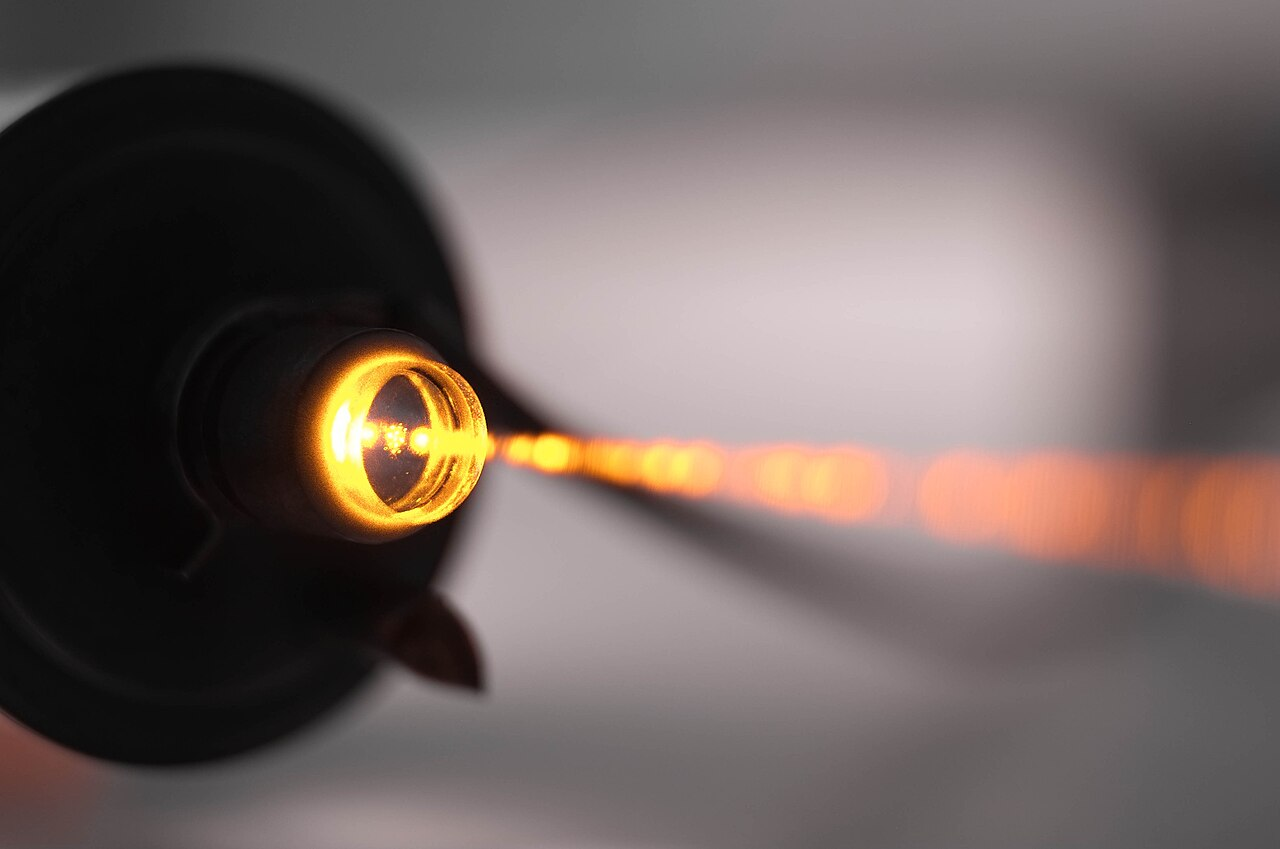
\includegraphics[width=0.58\linewidth]{images/book4/hene-laser-594nm.jpg}

{\small 氦氖激光管在 \qty{594}{nm} 黄线处发光：管内放电的辉光，以及经输出镜射出的光束。照片：Telementor, CC~BY~4.0。}
\end{omfigure}

\section{问题：从激光管到月球的氦氖激光器}

\begin{problem}[{周末问题——一台激光器的搭建、表征与
应用}]\label{pb:b2:laser:1}
实验台上的\omterm{def:b2:laser:cavity}{激光器}：玻璃管 $L = \qty{30}{cm}$，孔径
\qty{1}{mm}，氦氖混合气体，放电 \qty{5}{mA}，电压为
\qty{1.5}{kV}；反射镜 $R_1 = 0.999$，$R_2 = 0.99$；波长
\qty{632.8}{nm}；输出 \qty{1}{mW}。数据：氦的亚稳态能级
位于 \qty{20.61}{eV}，氖的上激光能级位于 \qty{20.66}{eV}，
寿命为 \qty{100}{ns}，下激光能级位于 \qty{18.70}{eV}，
寿命为 \qty{10}{ns}；气体温度 \qty{400}{K}；氖的摩尔质量
\qty{20}{g/mol}；截面 $\sigma = \qty{3e-17}{m^2}$；$h =
\qty{6.63e-34}{J.s}$，$k_B = \qty{1.38e-23}{J/K}$，$k_BT$ 在 \qty{400}{K} 时
$= \qty{0.0345}{eV}$。

\textbf{第一部分——介质。}
\begin{enumerate}
  \item 激光谱线的光子能量与频率。
  \item 氦和氖的能级相差 \qty{0.05}{eV}：与
        $k_BT$ 比较，并说明碰撞转移 He $\to$ Ne 为何
        高效。
  \item 氖的上能级与基态的玻尔兹曼比，在
        \qty{400}{K} 且无放电时，并加以评论。
  \item 由两个寿命说明，一旦上能级得到补充，氖能级间的\omterm{prop:b2:laser:gain}{粒子数反转}
        为何易于维持。
  \item 谱线的多普勒宽度：氖原子在
        \qty{400}{K} 下的最可几速率，以及数量级上的 $\Delta\nu \approx \nu\,v/c$
        （精确式为 $\Delta\nu = 2\nu\sqrt{2k_BT\ln2/Mc^2}$）。
  \item 取 $\Delta N = N_2 - N_1 = \qty{3e15}{m^{-3}}$，求小信号
        增益系数，以及在 \qty{30}{cm} 上的单程增益。
\end{enumerate}

\textbf{第二部分——谐振腔。}
\begin{enumerate}[resume]
  \item 阈值增益系数；给出相对于第 6 题的余量。
  \item 纵模间距；能够振荡的纵模数目。
  \item 腔内功率与管孔中的腔内光强。
  \item 稳态时增益由什么决定，多余的
        泵能量去了哪里？
  \item 输入电功率与输出光功率：效率；
        说明其如此之低的两个原因。
  \item 起振：每往返一次的净增益 $2(g_0 - g_{\text{阈}})L$，
        稳态时腔内的光子数，一个光子的
        往返次数，以及起振时间。
  \item 管子升温并伸长 \qty{1}{\micro m}：某一纵模的
        频移，及其对单模\omterm{def:b2:laser:cavity}{激光器}的影响。
  \item 管两端以\omterm{prop:b2:wave-interfaces:brewster}{布儒斯特角}窗片封闭：这对输出光的
        偏振有何影响？为何它不引入
        损耗？
\end{enumerate}

\textbf{第三部分——光束。}
\begin{enumerate}[resume]
  \item 谐振腔产生\omterm{prop:b2:laser:gaussian}{束腰} $w_0 = \qty{0.3}{mm}$：求\omterm{prop:b2:laser:gaussian}{瑞利
        长度}、发散角，以及距\omterm{prop:b2:laser:gaussian}{束腰} \qty{10}{m} 处的光束直径。
  \item 出口处的峰值光强；与阳光
        （\qty{1}{kW/m^2}）相比较。
  \item 焦距为 $f = \qty{50}{mm}$ 的透镜：焦点处的\omterm{prop:b2:laser:gaussian}{束腰}与
        峰值光强。
  \item 光束射入眼睛（焦距 \qty{17}{mm}）：视网膜上的光斑
        大小与光强；对于 \qty{1}{mW}，眨眼为何不算太慢，
        以及“2 类”的含义是什么。
  \item $\times 10$ 扩束器：新的发散角与光斑直径，
        位于 \qty{1}{km} 处。
  \item \omterm{prop:b2:scalar-light-model:coherence}{相干长度}：若\omterm{def:b2:laser:cavity}{激光器}工作于单一纵模，其宽度为
        \qty{1}{MHz}；若工作于跨越 \qty{1}{GHz} 的三个纵模，则\omterm{prop:b2:scalar-light-model:coherence}{相干长度}分别为多少？
\end{enumerate}

\textbf{第四部分——奔向月球。}
测距站发射 \qty{100}{mJ} 能量的脉冲，脉宽 \qty{100}{ps}，波长
为 \qty{532}{nm}，经口径 \qty{1}{m} 的望远镜发出；大气将出射
光束展宽到 \qty{1}{''}（$\qty{4.8e-6}{rad}$）。
\begin{enumerate}[resume]
  \item 每个脉冲的光子数与峰值功率。
  \item 月球上的光斑半径（距离 \qty{3.8e8}{m}）；与
        \omterm{def:b2:diffraction:huygens}{衍射}极限光斑作比较。
  \item 面积为 \qty{0.1}{m^2} 的反射器阵列截获脉冲的
        多大比例，截获多少光子？
  \item 阵列的 \qty{4}{cm} 角锥棱镜以 $\lambda/d$ 的扩散角返回光，
        求地球上的光斑半径、被望远镜截获的比例，
        以及每个脉冲探测到的光子数
        （取总光学效率为 $0.1$）。
  \item 往返时间约为 \qty{2.56}{s}，测量精度为
        \qty{100}{ps}：每个脉冲的距离精度；经过 $10^4$
        次返回之后，与月球每年远离 \qty{3.8}{cm} 的
        速率相比较。
\end{enumerate}
\end{problem}
